% !TeX spellcheck = en_US
\chapter{Vacuum robot}

The dream of having a robot in our houses doing all tedious work has been around for a long time. \citeaus{gates2007} predicts that robots will soon be in every home. Despite the huge need and significant engineering efforts, these robots are available to the market slower than expected. This chapter overviews domestic cleaning robots in general, vacuum robots and one of the engineering challenge, \ie, coverage path planning.

\section{Domestic Cleaning Robots}
\label{sec:cleaning_robots}

Cleaning robots have huge business potential. There are countless possible domestic applications for robots: floor vacuuming, mopping, kitchen and bathroom cleaning, dish washing, lawn mowing, \etc. Nearly half of those applications involve cleaning. Within all cleaning tasks, around one eighth relates to vacuuming \cite{cakmak2013hri}. For professional cleaning service, the market share in Europe alone was worth billions of USD \cite{schofield1995}. In 2020, 21.6~millions units of domestic robots, worth 5 billions USD in sales value, are sold worldwide \cite{ifr}. Despite this potential and around 20 years of research and development, in terms of efficiency and cost, cleaning robots could not yet fully replace the need of manual labour works \cite{siciliano2016}.\\

Having attracted a lot of academic attention for a long time, cleaning robots are still technically challenging. \citeausm{prassler2016} list related technical problems: absolute positioning, dynamic environments, human-robot interaction, power supply, \etc. Separately, all of these problems either have proposed approaches or tested solutions. However, they usually work in theoretical rather than real-world conditions, especially from a cost point-of-view. Companies often find themselves either reinvent or adapt to their own industrial needs. \cite{prassler2016}\\

\citeausm{kim2019ijars} give an overview on the directions of recent researches for future cleaning robots. While most of these current models are still constrained to two-dimensional workspace, some researchers focus on multi-purpose cleaning robots for the future (\figref{fig:okada2006_1}). Their goal is to handle furnitures, non-flat surfaces and diverse tasks. These advance robots would involve more learning-based approaches: learning from demonstration, supervised learning, reinforcement learning, \etc. \cite{kim2019ijars}

\begin{figure}[!htb]
	\centering
	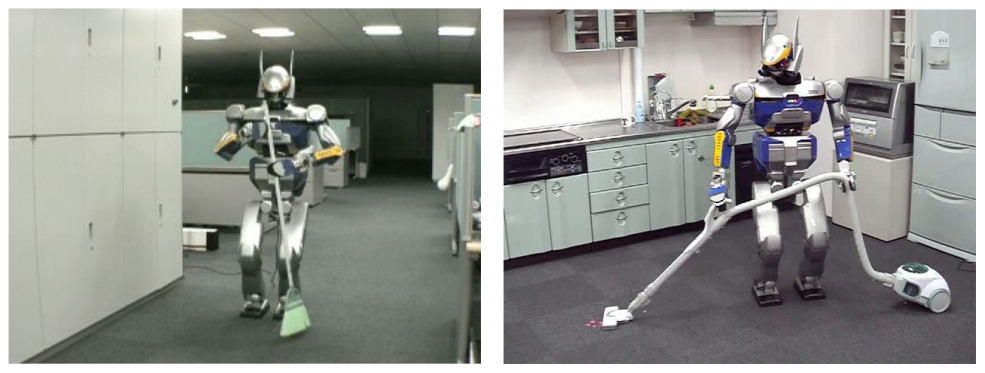
\includegraphics[width = 0.7\textwidth]{okada2006_1.png}
	\caption{Multi-purpose cleaning robot \cite{okada2006}.}
	\label{fig:okada2006_1}
\end{figure}

\section{Vacuum Robots}
\label{sec:vacuum_robots}

Comparing to other domestic chores, floor vacuuming is more challenging. In other tasks, \eg, cleaning of pool, solar panel or window, the robots usually handle static and known space. The environment is mostly two-dimensional, sometimes requires fixed obstacle avoidance. Vacuum robots have to deal with more diverse environment settings, \eg, unknown map, dynamic obstacles, interaction with human. In addition, many customers lack willingness to make physical changes to their rooms for the robots \cite{vaussard2014ras}.

\subsection{Design Characteristics}
Early 2000s, some major ground works on coverage problem were laid down \cite{huang1986icra, zelinsky1993icar, choset2000ar, gabriely2002icra}. Before the end of 2005, many major companies released their first models of domestic cleaning robots \cite{siciliano2016}. Most of these models and even current ones still have a lot in common:
\begin{itemize}
	\setlength\itemsep{0em}
	\item Shape: Round-shaped
	\item Dimension: Varies in height, diameter around 30-40 cm
	\item Cleaning technology: One suction pump (as the main \ac{EE} tool) and side brush (as supporting tool)
	\item Common sensors: Sonar, bumper and cliff (stair avoidance) sensors
	\item Coverage strategy: Bang and bounce (random motion), contour following
\end{itemize}

Most early models have round shape. The suction pump is limited between the two wheels. Another used design is D-shaped robot (\figref{fig:neato}), enabling wider brush and more corner coverage.

\begin{figure}[!htb]
	\centering
	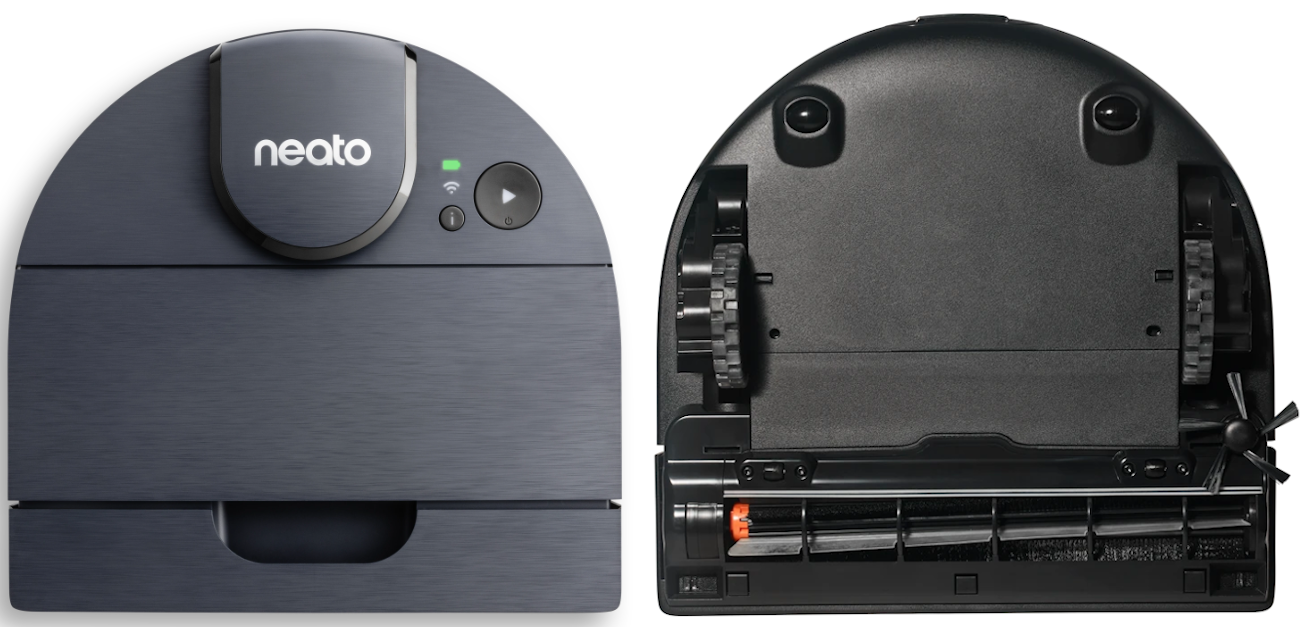
\includegraphics[width = 0.55\textwidth]{neato.png}
	\caption{Neato Robotics: Neato D8 \cite{neato}.}
	\label{fig:neato}
\end{figure}

Even though it is better to have knowledge of surrounding environment, domestic robots generally have the minimum amount of sensors. A \$20 sensor is very expensive for a robot that should cost around \$300-400. However, there are still exceptional cases. Costing \$3400 , Ottoro has two digital cameras, 12 pairs of ultrasonic sensor and highly sensitive air bumper (\figref{fig:ottoro}). With all state-of-the-art technologies, the robot could identify its position with the accuracy of $\pm$3cm and follow better coverage strategies. \cite{siciliano2016}

\begin{figure}[!htb]
	\centering
	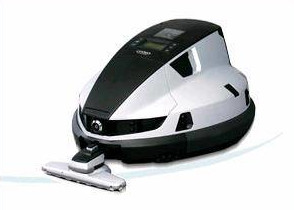
\includegraphics[width = 0.4\textwidth]{ottoro.jpg}
	\caption{Hanool Robotics: Ottoro \cite{ottoro}.}
	\label{fig:ottoro}
\end{figure}

Early robot models use simple approaches to coverage problem, \ie, \textit{Bang and Bounce}. With only a bumper sensor at the front, this strategy changes the robot direction whenever it hits an obstacle. Despite not guaranteeing complete coverage, this strategy converges to good space coverage after a large amount of time (\figref{fig:liu2008wcica_1}) \cite{liu2008wcica}. Some models integrate with contour following, achieved by adding sensor on the robot side for wall detection. As users are expecting more intelligent robots, a random motion is hardly appealing any longer \cite{goel2013iros}.

\begin{figure}[!htb]
	\centering
	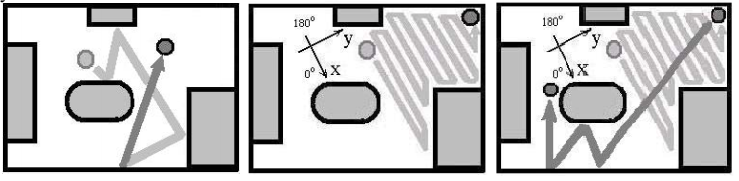
\includegraphics[width = 0.7\textwidth]{liu2008wcica_1.png}
	\caption{Random and fixed motion mode \cite{liu2008wcica}.}
	\label{fig:liu2008wcica_1}
\end{figure}

\subsection{Cost}
Whether a cleaning robot would be a business success or failure depends heavily on its cost. Early models, with the costs from \texteuro 800-1750, were 10-20 times more expensive than a high-quality vacuum cleaner. Despite the high cost, many were frequently trapped by electrical cables and need monthly repairs. This led to the lack of trust from customers in the autonomy of these robots \cite{vaussard2014ras}. The first robot successfully entering the domestic market was Roomba from iRobot. Its success was not due to its performance, rather the affordable price, \ie \texteuro 350. To take advantage of this market potential, next generation robots should consider not only engineering improvements, but also customer perceptions. \cite{gutmann2012arso, royakkers2015ijsr, siciliano2016}

\section{Coverage Path Planning}

\subsection{Introduction}

\ac{CPP} is the problem of finding the most optimal path to fully cover an area. Given a robot description and a map to cover, the output is a robot trajectory. \citeausm{huang1986icra} first describe the problem and its usage for robotic lawnmowers. Early seminal works formalize the coverage problem and propose new algorithms that prioritize coverage completeness \cite{latombe1991, zelinsky1993icar, choset2000ar}. In recent years, researchers have focused on other aspects of the coverage problem, \eg, extending it to dynamic or 3D environments, accounting for kinematic constraints, planning for several robots.\\

One application of coverage algorithm is for vacuum robots, which has huge business potential \cite{schofield1995, ifr}. The market is currently very competitive with many technological innovations and diverse robot approaches. Traditional round-shaped robot models are easy with to plan with, but have trouble cleaning along the floor edges and corners thoroughly. Other products try to clean better along the edges by resorting to a D-shaped robot, although it is more difficult to navigate with.\\

In practice, two issues often arise when planning coverage paths that have often been abstracted away in the literature: the need to account for the precise robot shape with \ac{EE} placement, and a lack of unified metrics for algorithm performance. My thesis examines in details these two issues for robot with asymmetric \ac{EE}.\\

\subsection{Classification}

Classification of \ac{CPP} takes form in many criteria, the most common ones and their corresponding classes are as follows:

\begin{itemize}
	\item Based on problem characteristics:
	\begin{itemize}
		\item Offline or Online: Offline algorithm assumes full prior knowledge of a static environment. Online algorithm do not make that assumption. As most online approaches utilize data from real-time sensor, they are also known as sensor-based coverage algorithms.
		\item With or without kinematics constraints: whether the robots could easily rotate in place or have a minimum turn radius.
	\end{itemize}
	\item Based on solution characteristics:
	\begin{itemize}
		\item Heuristics or Complete: whether the algorithms guarantee complete coverage of space.
		\item Type of environment decomposition: exact, approximate or semi-approximate cellular decomposition.
	\end{itemize}	
\end{itemize}

This subsection introduces some well-known coverage approaches.

\subsubsection{Trapezoidal Decomposition \ac{CPP}}
\citeaus{latombe1991} introduces the simplest offline exact cellular decomposition for 2D map. He assumes that map and obstacles are polygonal. When touching a obstacle vertex point, the swiping line divides the map into trapezoidal cells. One downside of this decomposition approach is to generate some redundant cells. \Eg, in \figref{fig:galceran2013ras_1}, the 9th and 11th cells can be grouped to one single cell. The less nodes there are, the easier it is to solve the associated \ac{TSP}.

\begin{figure}[!htb]
	\centering
	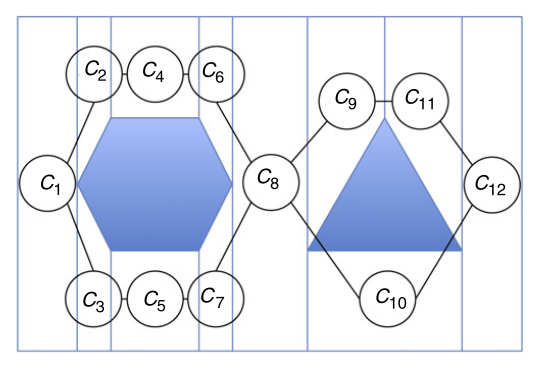
\includegraphics[width = 0.5\textwidth]{galceran2013ras_1.png}
	\caption{Trapezoidal decomposition with polygonal space and obstacles \cite{galceran2013ras}.}
	\label{fig:galceran2013ras_1}
\end{figure}

\subsubsection{Boustrophedon Decomposition \ac{CPP}}
\citeaus{choset2000ar} reduces the number of unnecessary cells. New cells are created only in an \textit{event}, when a cell is split into many or when cells are merged into one (\figref{fig:choset2000ar_1}). In such \textit{event}, the intersection point between the swiping line and obstacle boundary is a \textit{critical point}. The word \textit{boustrophedon} implies the simple zig-zag coverage pattern. The author also notes that using boustrophedon pattern alone is prone to incomplete coverage. The robot specifically misses areas around the obstacle perimeters, which are not parallel to the moving direction.

\begin{figure}[!htb]
	\centering
	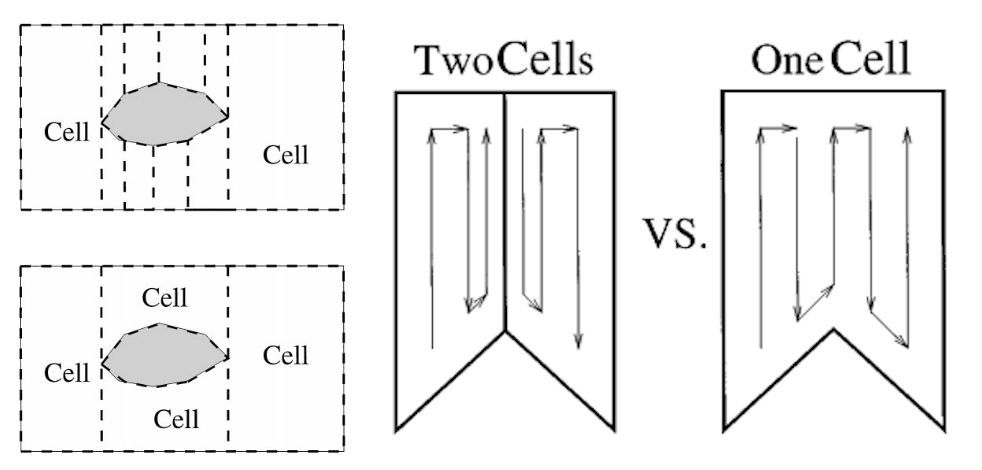
\includegraphics[width = 0.7\textwidth]{choset2000ar_4.png}
	\caption{Having less cells by creating new ones only in split or merge event.}
	\label{fig:choset2000ar_1}
\end{figure}

\subsubsection{Decomposition in terms of Critical Points of Morse Functions}
Previous presented approaches decompose the map using a line. \citeausm{choset2000icra} generalize the shape of the slice by changing its functional definition, called Morse function. For Boustrophedon Decomposition, the slice function of a line is $h(x)=x$, where $x$ is the first coordinate in 2D space. Different Morse functions induce different cell shapes and their corresponding coverage patterns (\figref{fig:choset2000icra_1}). Different problem settings may fit better with one coverage pattern than the others. \citeaus{acar2001iros} later develop an online \ac{CPP} algorithm using Morse function based decomposition.

\begin{figure}[!htb]
	\centering
	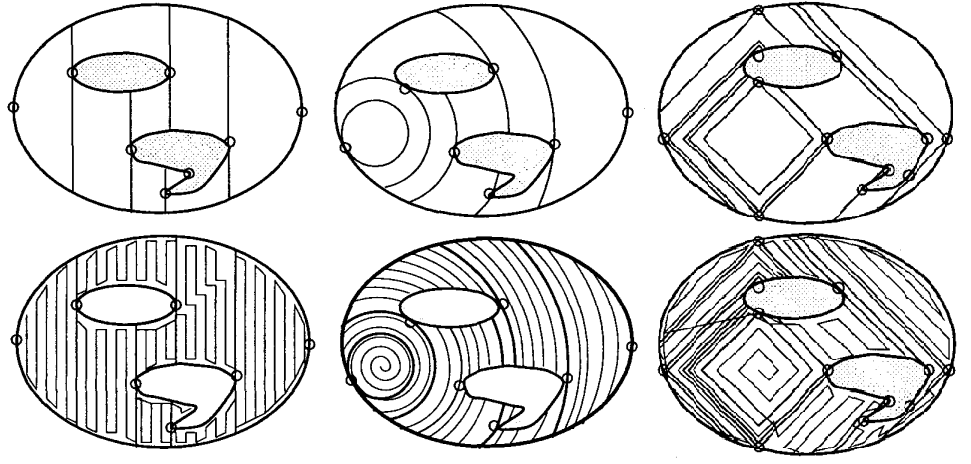
\includegraphics[width = 0.7\textwidth]{choset2000icra_1.png}
	\caption{Boustrophedon, spiral, diamond cell decompositions and coverage patterns~\cite{choset2000icra}.}
	\label{fig:choset2000icra_1}
\end{figure}

\subsubsection{Wavefront \ac{CPP} Algorithm}
\citeausm{zelinsky1993icar} use a completely different branch of approaches to CPP. They adopt their approach for \ac{PP} problem \cite{zelinsky1991}, to create a numeric potential field over the map using the distance transform. The distance wave increases in value as it spreads from goal point to neighbouring grid cells, until every cell is reached. If the robot follows a gradient-descent path, it is the shortest path from start to end point. On the other hands, if the robot follows a gradient-ascent path, it visits all cells and covers the whole map (\figref{fig:zelinsky1993_2}). To reduce high number of turns in \textit{distance transform}, the authors propose to add the distance from walls and obstacles to the potential field, resulting the \textit{path transform} trajectory. The approach is offline and allows start and end points to be specified.

\begin{figure}[!htb]
	\centering
	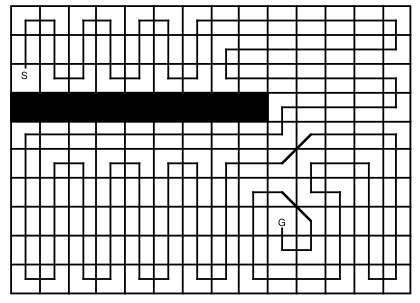
\includegraphics[width = 0.5\textwidth]{zelinsky1993_2.png}
	\caption{Complete coverage path.}
	\label{fig:zelinsky1993_2}
\end{figure}

\subsubsection{Spiral-STC Grid-based \ac{CPP} Algorithm}
\citeaus{gabriely2002icra} propose an online algorithm guaranteeing complete coverage of all free accessible subcells. They first divide the map into large cells, and each one of them contains four small subcells. At each position, the robot explores neighbouring large cell in a certain direction (counter clockwise). As large cells are visited, the spanning tree connecting them extends a new branch. This process iterates until the robot visits all possible large cells. In this exploration stage, the robot has travelled only on one side of the spanning tree. Then, the robot turns back and traverses on the other side of the tree to cover the rest of the map (\figref{fig:gabriely2002icra_2}).

\begin{figure}[!htb]
	\centering
	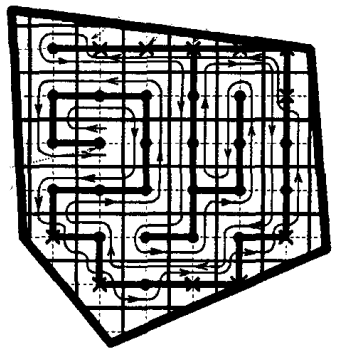
\includegraphics[width = 0.35\textwidth]{gabriely2002icra_2.png}
	\caption{An execution of full Spiral-STC.}
	\label{fig:gabriely2002icra_2}
\end{figure}

\subsubsection{Neural Network Approach to CPP}
The online \ac{CPP} approach by \citeaus{yang2004tsmc} is inspired by neural networks. Each cell in the grid map also represents a neuron in the network. The receptive field of each cell is only its 8 neighbours. Each neuron has a shunting dynamic equation. Certain thresholds over the shunting inputs allow the positive neural activities (pull activities from free spaces) to spread across the map, while limit the negative neural activities (push activities from obstacles) to stay in each local area. To limit the number of turns, the robot path takes both neural activity and previous poses into account. In the end, it also results in a potential field, similar to the one in \citeauthor*{zelinsky1993icar}'s work (\figref{fig:yang2004_3}). This approach can deal with dynamic and unstructured obstacles. However, unlike other online algorithms, \eg, \cite{butler2000, acar2001iros, gabriely2002icra}, for the network setup, the map size must be known a priori.

\begin{figure}[!htb]
	\centering
	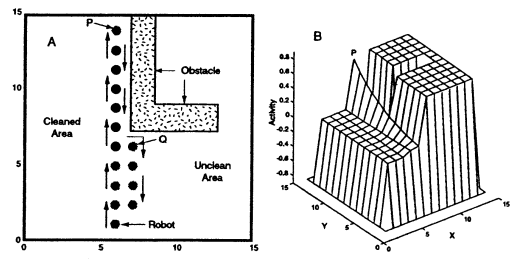
\includegraphics[width = 0.7\textwidth]{yang2004_3.png}
	\caption{Robot path and the activity landscape \cite{yang2004tsmc}.}
	\label{fig:yang2004_3}
\end{figure}

\subsubsection{Convex Sensor Placement Problem to \ac{CPP}}
\citeausm{arain2015icra} solve the convex sensor placement problem by formulating a novel directed graph on top of the grid map. Each cell has four nodes, corresponding to four poses. Each node has connections with other nodes in the same grid cell and one node in the neighbouring cell of the same direction. \Eg, if the current node represents the pose going up, it connects with the node going up in the above grid cell, if that exists (\figref{fig:arain2015icra_1}). As an area inspection problem, the range of the end-effector (a gas detection sensor) is much greater than the size of each grid cell. The coverage problem is similar to the \ac{CSP}, which doesn't require to visit all nodes in the graph. The authors find a path traversing the graph using iterative convex relaxation method (\figref{fig:arain2015icra_2}).

\begin{figure}[!htb]
	\centering
	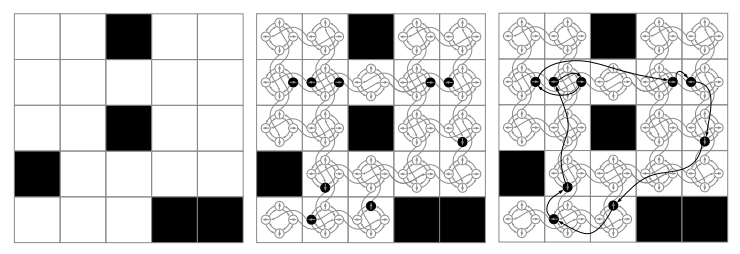
\includegraphics[width = 1\textwidth]{arain2015icra_2.png}
	\caption{Trajectory from traversing the graph.}
	\label{fig:arain2015icra_2}
\end{figure}

\subsubsection{Turn-minimizing Coverage}
The offline algorithm of \citeaus{vandermeulen2019icra} resembles the line-sweep-based decomposition \cite{huang2001icra}, but for grid-based approach. The authors consider the problem as a \ac{TSP} instance. A \textit{rank} is similar to a sweep line and is a node in the \ac{TSP}. The robot covers the map by visiting all interior and perimeter ranks (\figref{fig:vandermeulen2019icra_5}). Each rank has three vertices: two end points and a midpoint. As the cost from the midpoint vertex to vertices in other ranks is infinity, it enforces the robot to go from one end to the others within a rank.

\begin{figure}[!htb]
	\centering
	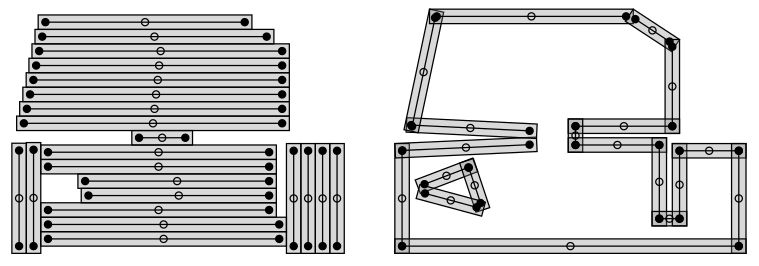
\includegraphics[width = 0.79\textwidth]{vandermeulen2019icra_5.png}
	\caption{Interior and perimeter ranks. \cite{vandermeulen2019icra}.}
	\label{fig:vandermeulen2019icra_5}
\end{figure} 

\clearpage